\section{main.c File Reference}
\label{main_8c}\index{main.c@{main.c}}
{\tt \#include $<$msp430x16x.h$>$}\par
{\tt \#include $<$stdio.h$>$}\par
{\tt \#include $<$stdlib.h$>$}\par
{\tt \#include $<$signal.h$>$}\par
{\tt \#include \char`\"{}ueaclib.h\char`\"{}}\par
{\tt \#include \char`\"{}ueac.h\char`\"{}}\par
{\tt \#include \char`\"{}external\_\-flash.h\char`\"{}}\par
{\tt \#include \char`\"{}interpreter.h\char`\"{}}\par
{\tt \#include \char`\"{}filter.h\char`\"{}}\par
{\tt \#include \char`\"{}conversion.h\char`\"{}}\par
{\tt \#include \char`\"{}global.h\char`\"{}}\par
{\tt \#include \char`\"{}timer.h\char`\"{}}\par
{\tt \#include \char`\"{}calibrate.h\char`\"{}}\par


Include dependency graph for main.c:\begin{figure}[H]
\begin{center}
\leavevmode
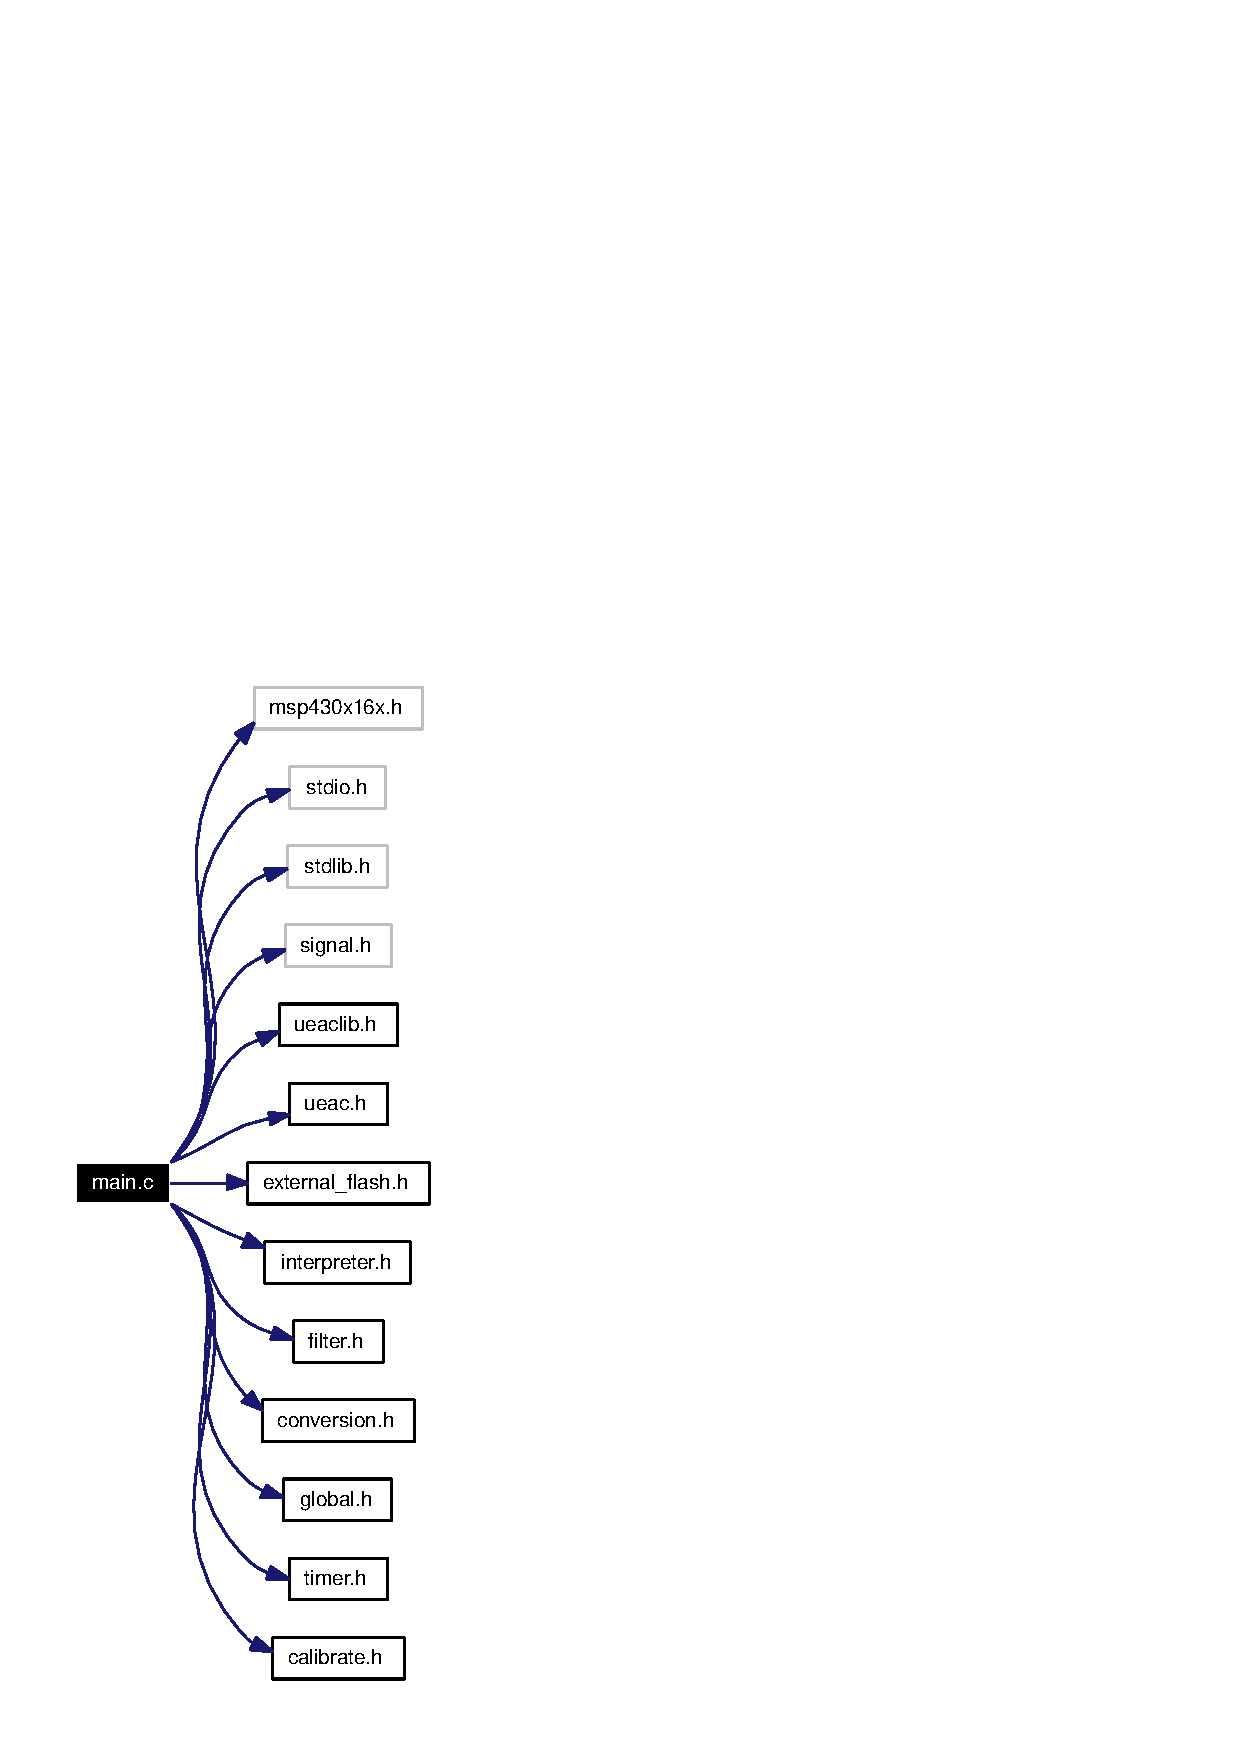
\includegraphics[width=103pt]{main_8c__incl}
\end{center}
\end{figure}
\subsection*{Functions}
\begin{CompactItemize}
\item 
void {\bf print\_\-grid\_\-v} ()
\item 
void {\bf print\_\-grid\_\-i} ()
\item 
int {\bf get\_\-command} (char $\ast$command\_\-buf)
\item 
int {\bf main} (void)
\item 
void {\bf scan\_\-probes} ()
\end{CompactItemize}
\subsection*{Variables}
\begin{CompactItemize}
\item 
short {\bf dac\_\-translation} [$\,$]
\end{CompactItemize}


\subsection{Function Documentation}
\index{main.c@{main.c}!get_command@{get\_\-command}}
\index{get_command@{get\_\-command}!main.c@{main.c}}
\subsubsection{\setlength{\rightskip}{0pt plus 5cm}int get\_\-command (char $\ast$ {\em command\_\-buf})}\label{main_8c_a3}




Definition at line 129 of file main.c.

References getchar().

Referenced by main().

\footnotesize\begin{verbatim}129                                    {
130   char ch;
131   int counter=0;
132   while(((ch=getchar())!='\n')&&(ch!='\r')&&(counter++<100)) {
133     *command_buf++=ch;
134   }
135   *command_buf++='\n';
136   *command_buf=0;
137   return (counter);
138 }     
\end{verbatim}\normalsize 




Here is the call graph for this function:\begin{figure}[H]
\begin{center}
\leavevmode
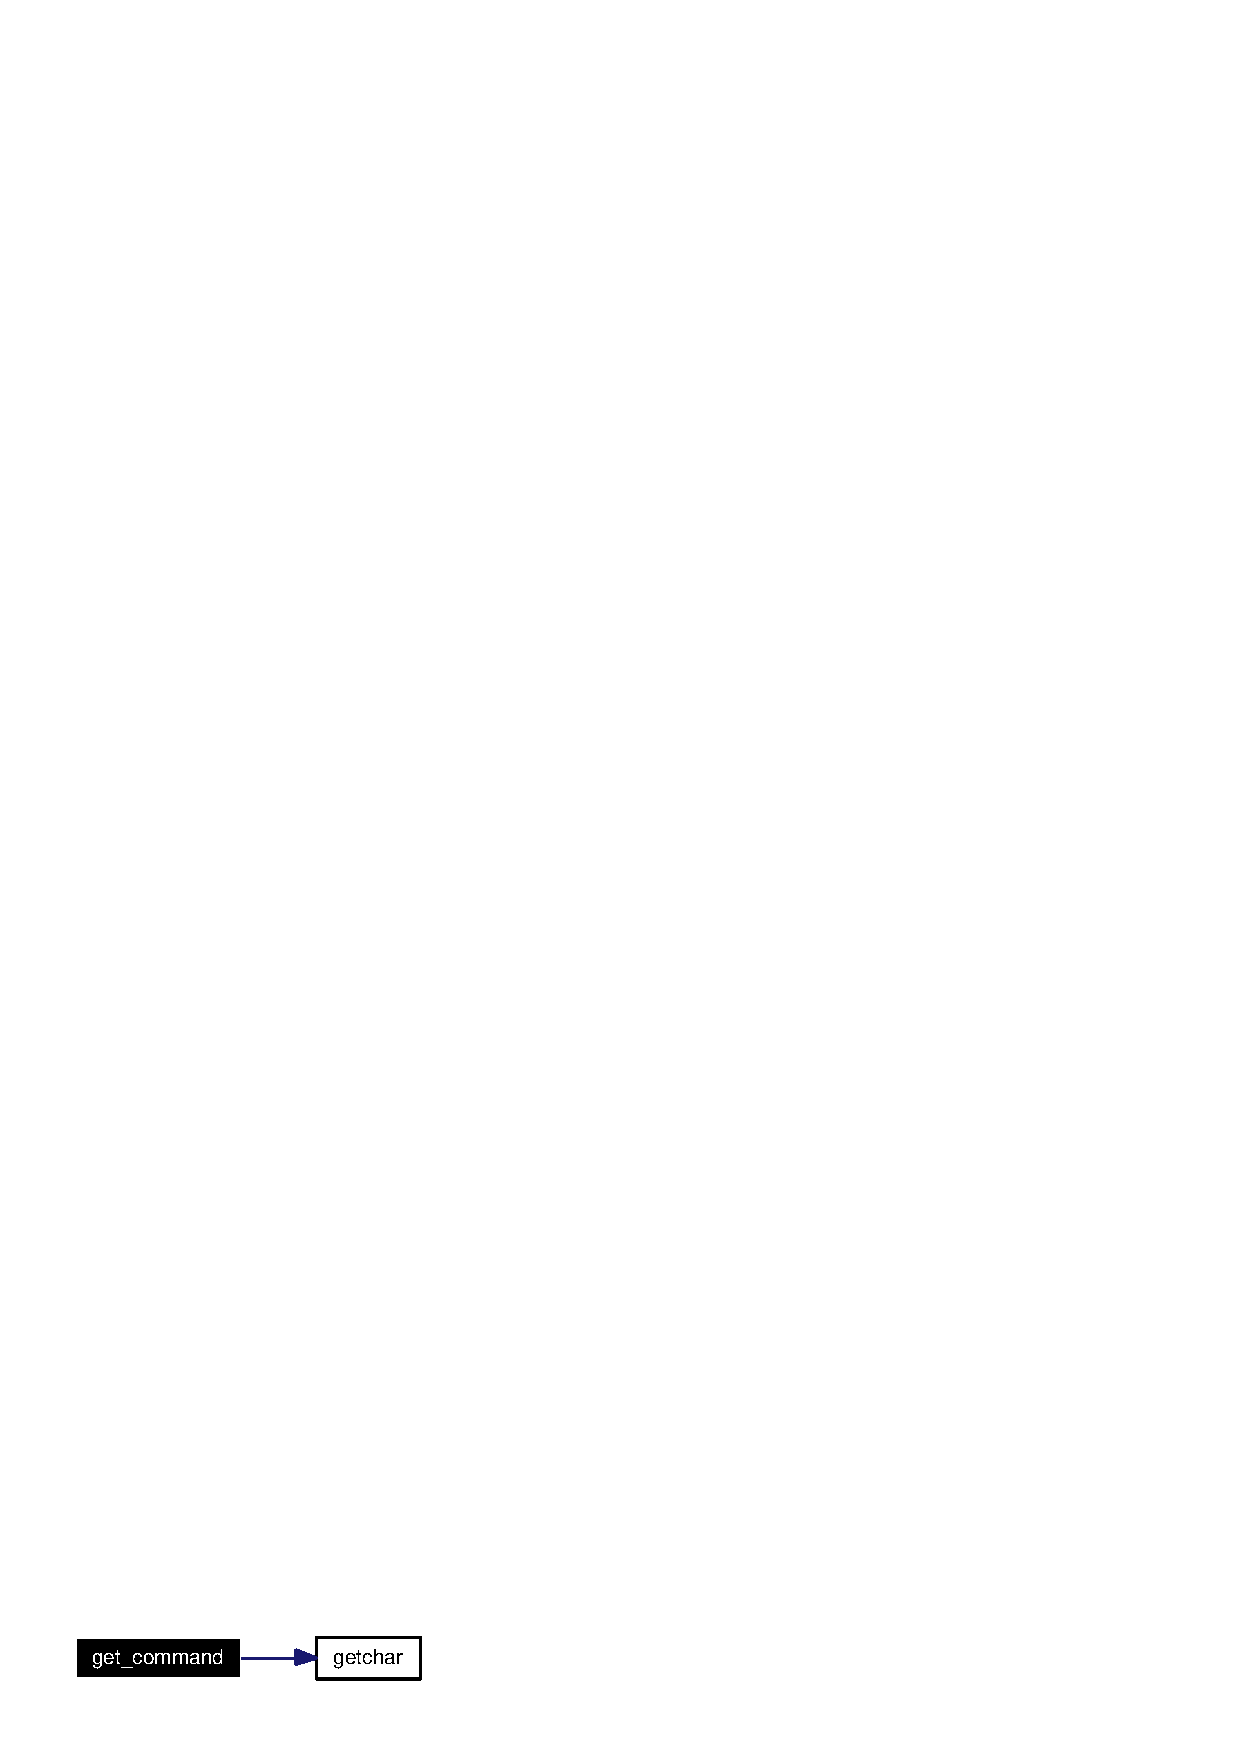
\includegraphics[width=101pt]{main_8c_a3_cgraph}
\end{center}
\end{figure}
\index{main.c@{main.c}!main@{main}}
\index{main@{main}!main.c@{main.c}}
\subsubsection{\setlength{\rightskip}{0pt plus 5cm}int main (void)}\label{main_8c_a4}




Definition at line 88 of file main.c.

References BACK\_\-WHITE, CLR, command, delay\_\-1\_\-25m\-S(), flash\_\-integrity\_\-test(), get\_\-command(), init\_\-global\_\-variables(), init\_\-sys(), interpreter(), led\_\-screen\_\-enable, scan\_\-leds(), ueac\_\-state, write\_\-current(), write\_\-led(), and write\_\-lla().

\footnotesize\begin{verbatim}88                {
89   int i;
90   init_sys();                        // setup the MSP430 peripherals
91   printf(BACK_WHITE);
92   printf(CLR);
93   printf("UEAC POST\n\r");
94   flash_integrity_test();
95   scan_leds();
96   init_global_variables();
97   for (i=0;i<25;i++) {
98     write_lla(i,0);
99     write_led(i,0);
100     write_current(i,0);
101   }
102   delay_1_25mS(800);     
103   printf(CLR);
104   printf("uEACos V2.2 base_002.9\n\r");
105   led_screen_enable=1;
106   while(1) {
107     printf("ueac> ");
108     get_command(command);
109     interpreter(command,&ueac_state);
110   }
111 }
\end{verbatim}\normalsize 




Here is the call graph for this function:\begin{figure}[H]
\begin{center}
\leavevmode
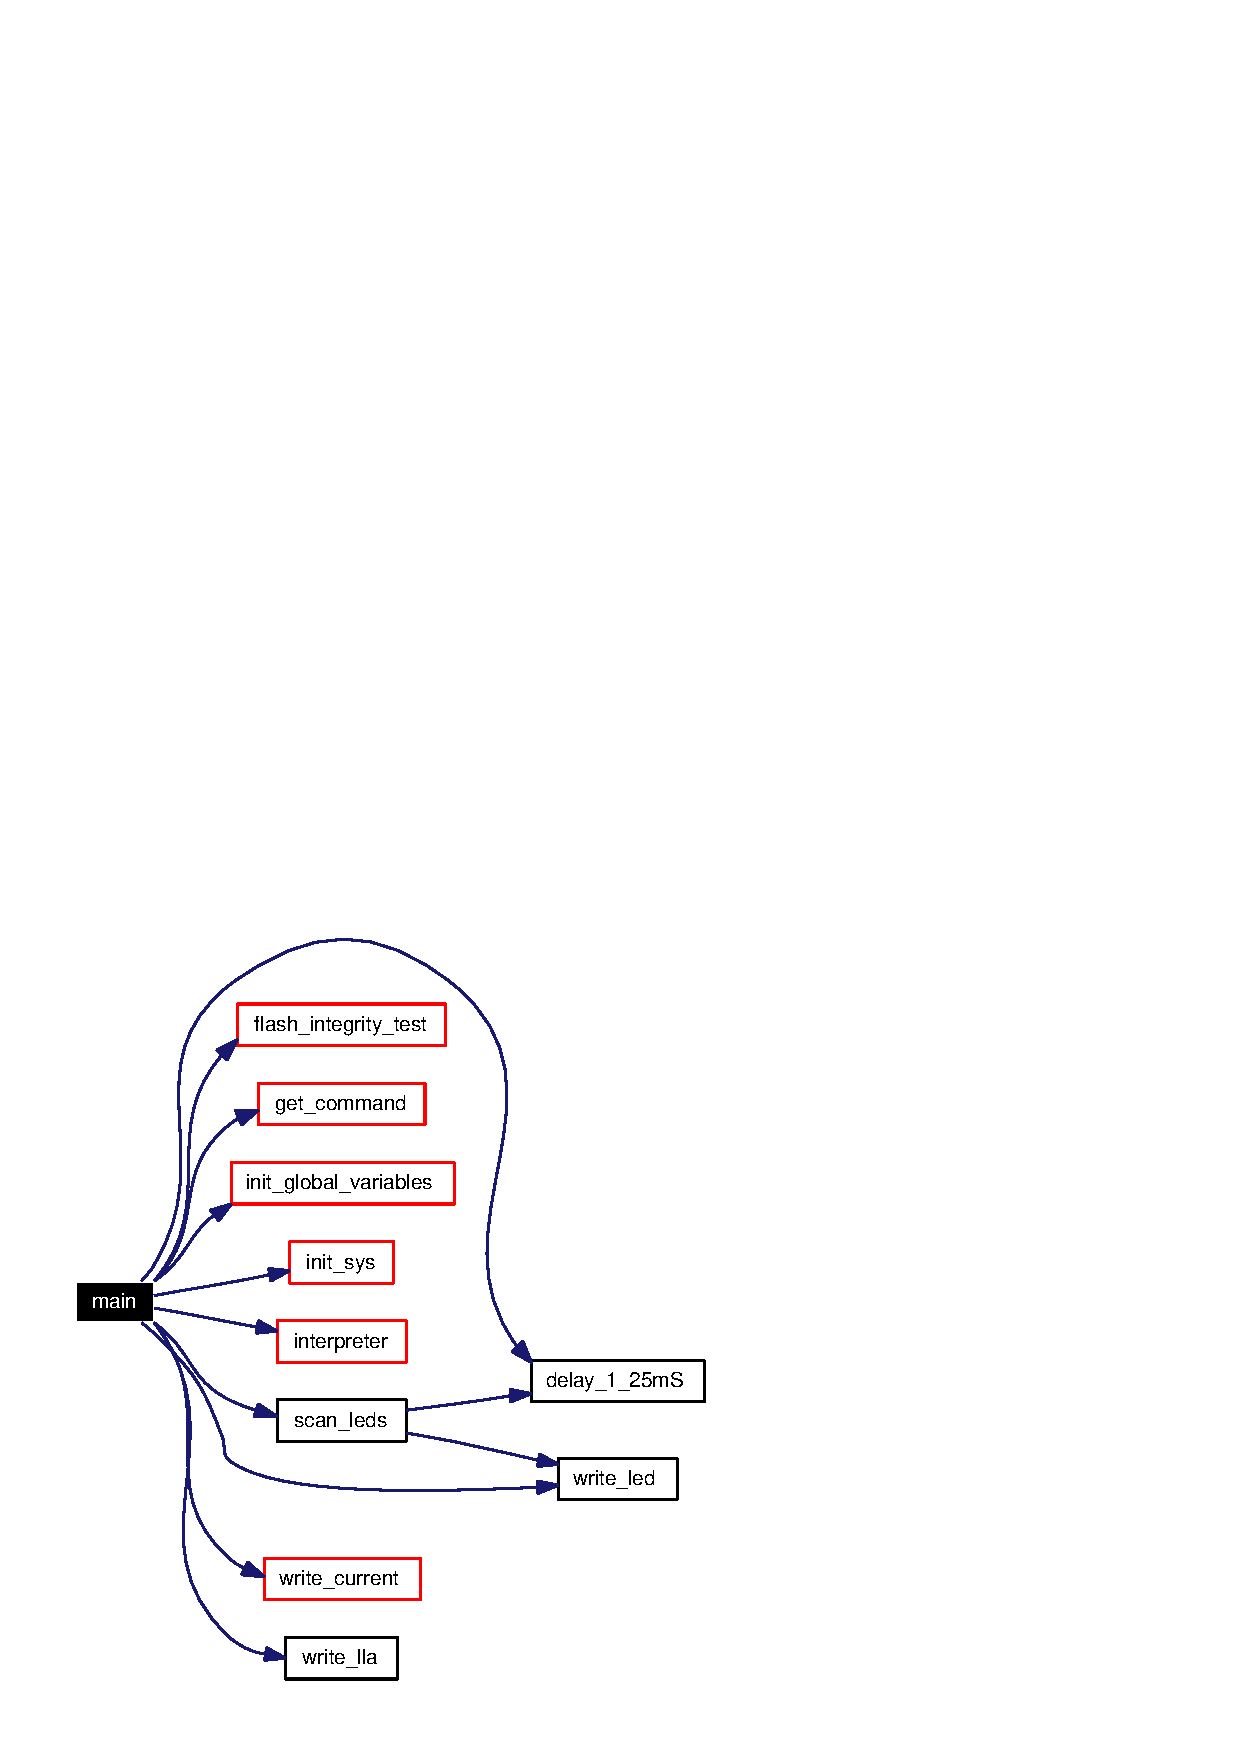
\includegraphics[width=169pt]{main_8c_a4_cgraph}
\end{center}
\end{figure}
\index{main.c@{main.c}!print_grid_i@{print\_\-grid\_\-i}}
\index{print_grid_i@{print\_\-grid\_\-i}!main.c@{main.c}}
\subsubsection{\setlength{\rightskip}{0pt plus 5cm}void print\_\-grid\_\-i ()}\label{main_8c_a2}




Definition at line 151 of file main.c.

References conversion\_\-result, convert\_\-a2d(), delay\_\-1\_\-25m\-S(), I\_\-CONVERSION, ueacval::integer, pin\_\-data, write\_\-current(), and write\_\-lla().

\footnotesize\begin{verbatim}151                     {
152   int i,j;
153   for (i=0;i<5;i++) {
154     for (j=0;j<5;j++) {
155       write_lla(i*5+j,1);
156       write_current(i*5+j,200);
157       delay_1_25mS(500);
158       convert_a2d(I_CONVERSION,pin_data[i*5+j].filtered_result,&conversion_result,i*5+j); 
159       printf("%d ",conversion_result.integer);
160       write_lla(i*5+j,0);
161     }
162     printf("\n\r");
163   }
164 }
\end{verbatim}\normalsize 




Here is the call graph for this function:\begin{figure}[H]
\begin{center}
\leavevmode
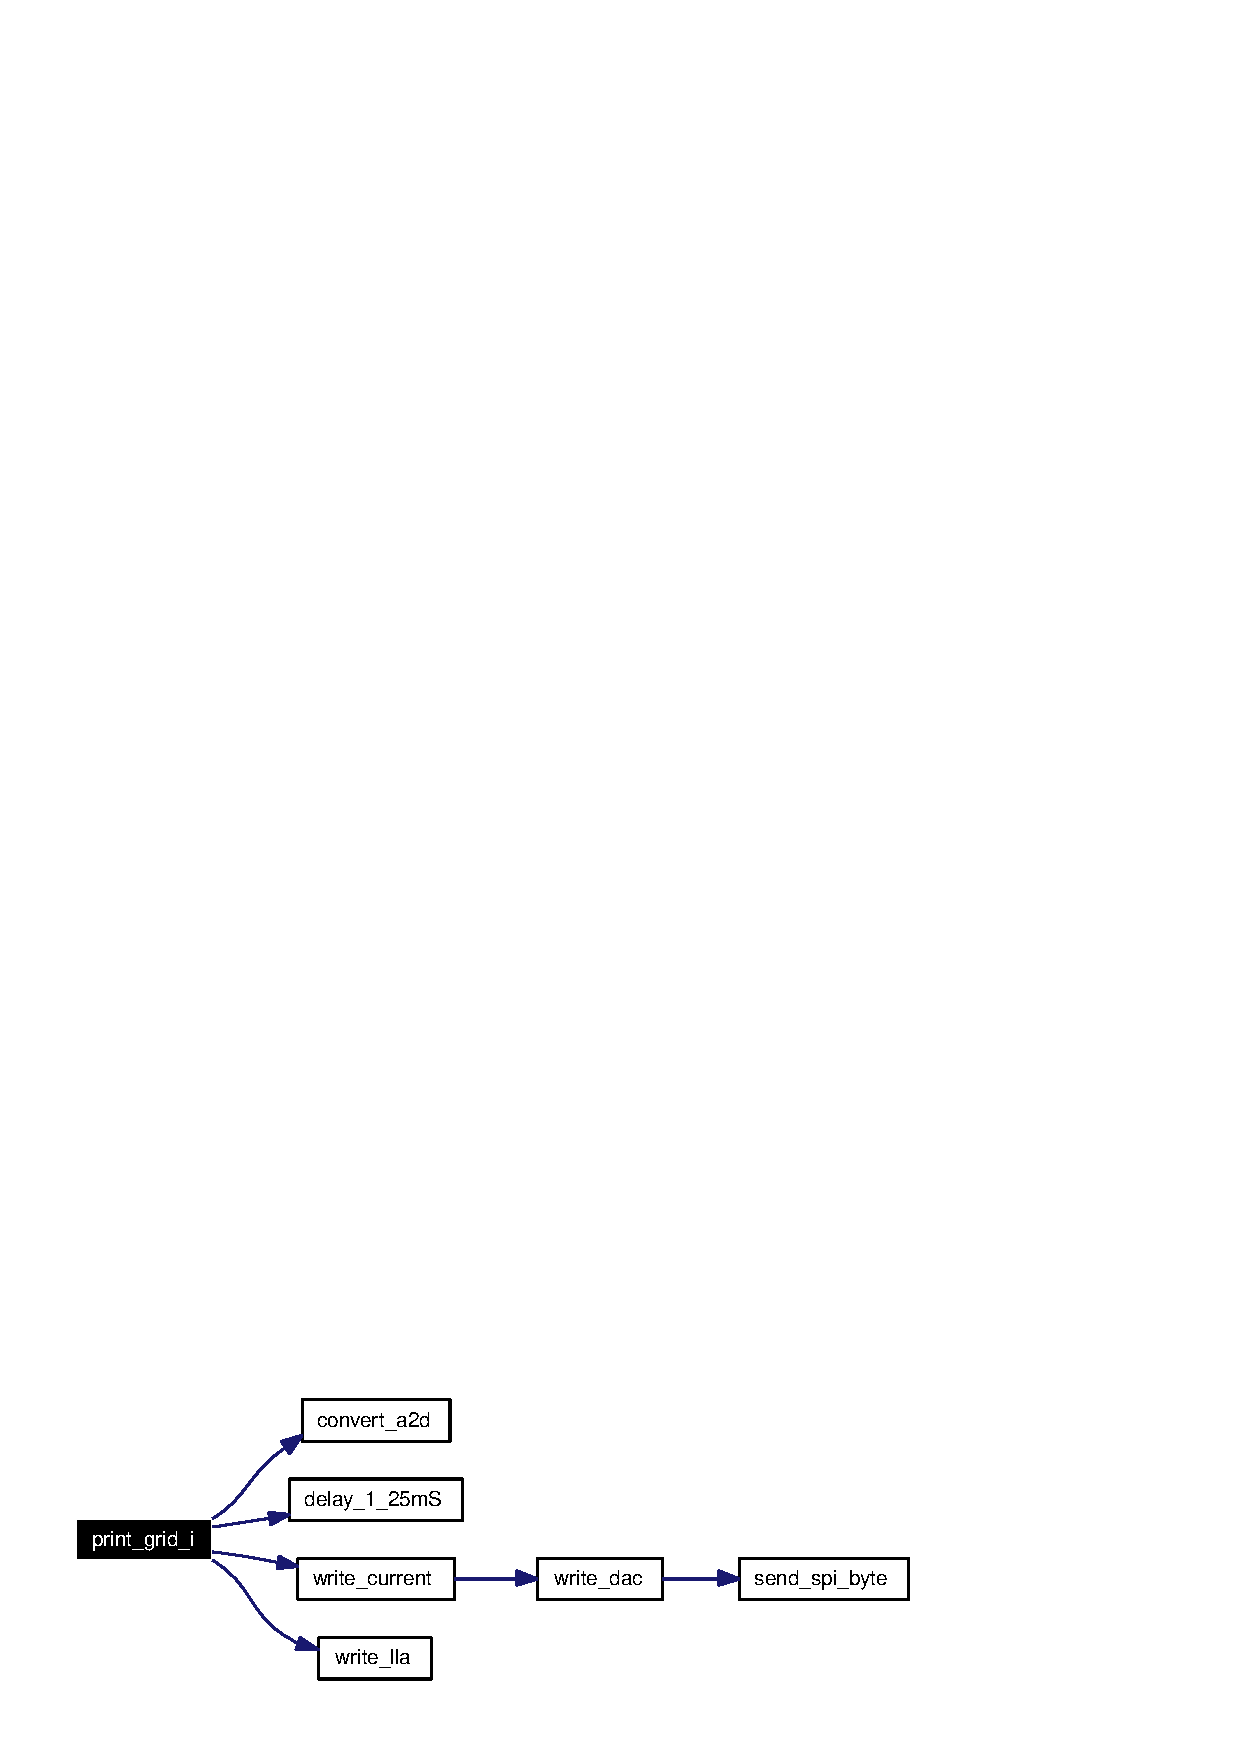
\includegraphics[width=218pt]{main_8c_a2_cgraph}
\end{center}
\end{figure}
\index{main.c@{main.c}!print_grid_v@{print\_\-grid\_\-v}}
\index{print_grid_v@{print\_\-grid\_\-v}!main.c@{main.c}}
\subsubsection{\setlength{\rightskip}{0pt plus 5cm}void print\_\-grid\_\-v ()}\label{main_8c_a1}




Definition at line 140 of file main.c.

References conversion\_\-result, convert\_\-a2d(), ueacval::hundredth, ueacval::integer, pin\_\-data, and V\_\-CONVERSION.

\footnotesize\begin{verbatim}140                     {
141   int i,j;
142   for (i=0;i<5;i++) {
143     for (j=0;j<5;j++) {
144       convert_a2d(V_CONVERSION,pin_data[i*5+j].filtered_result,&conversion_result,i*5+j); 
145       printf("%d.%d ",conversion_result.integer,conversion_result.hundredth);
146     }
147     printf("\n\r");
148   }
149 }
\end{verbatim}\normalsize 




Here is the call graph for this function:\begin{figure}[H]
\begin{center}
\leavevmode
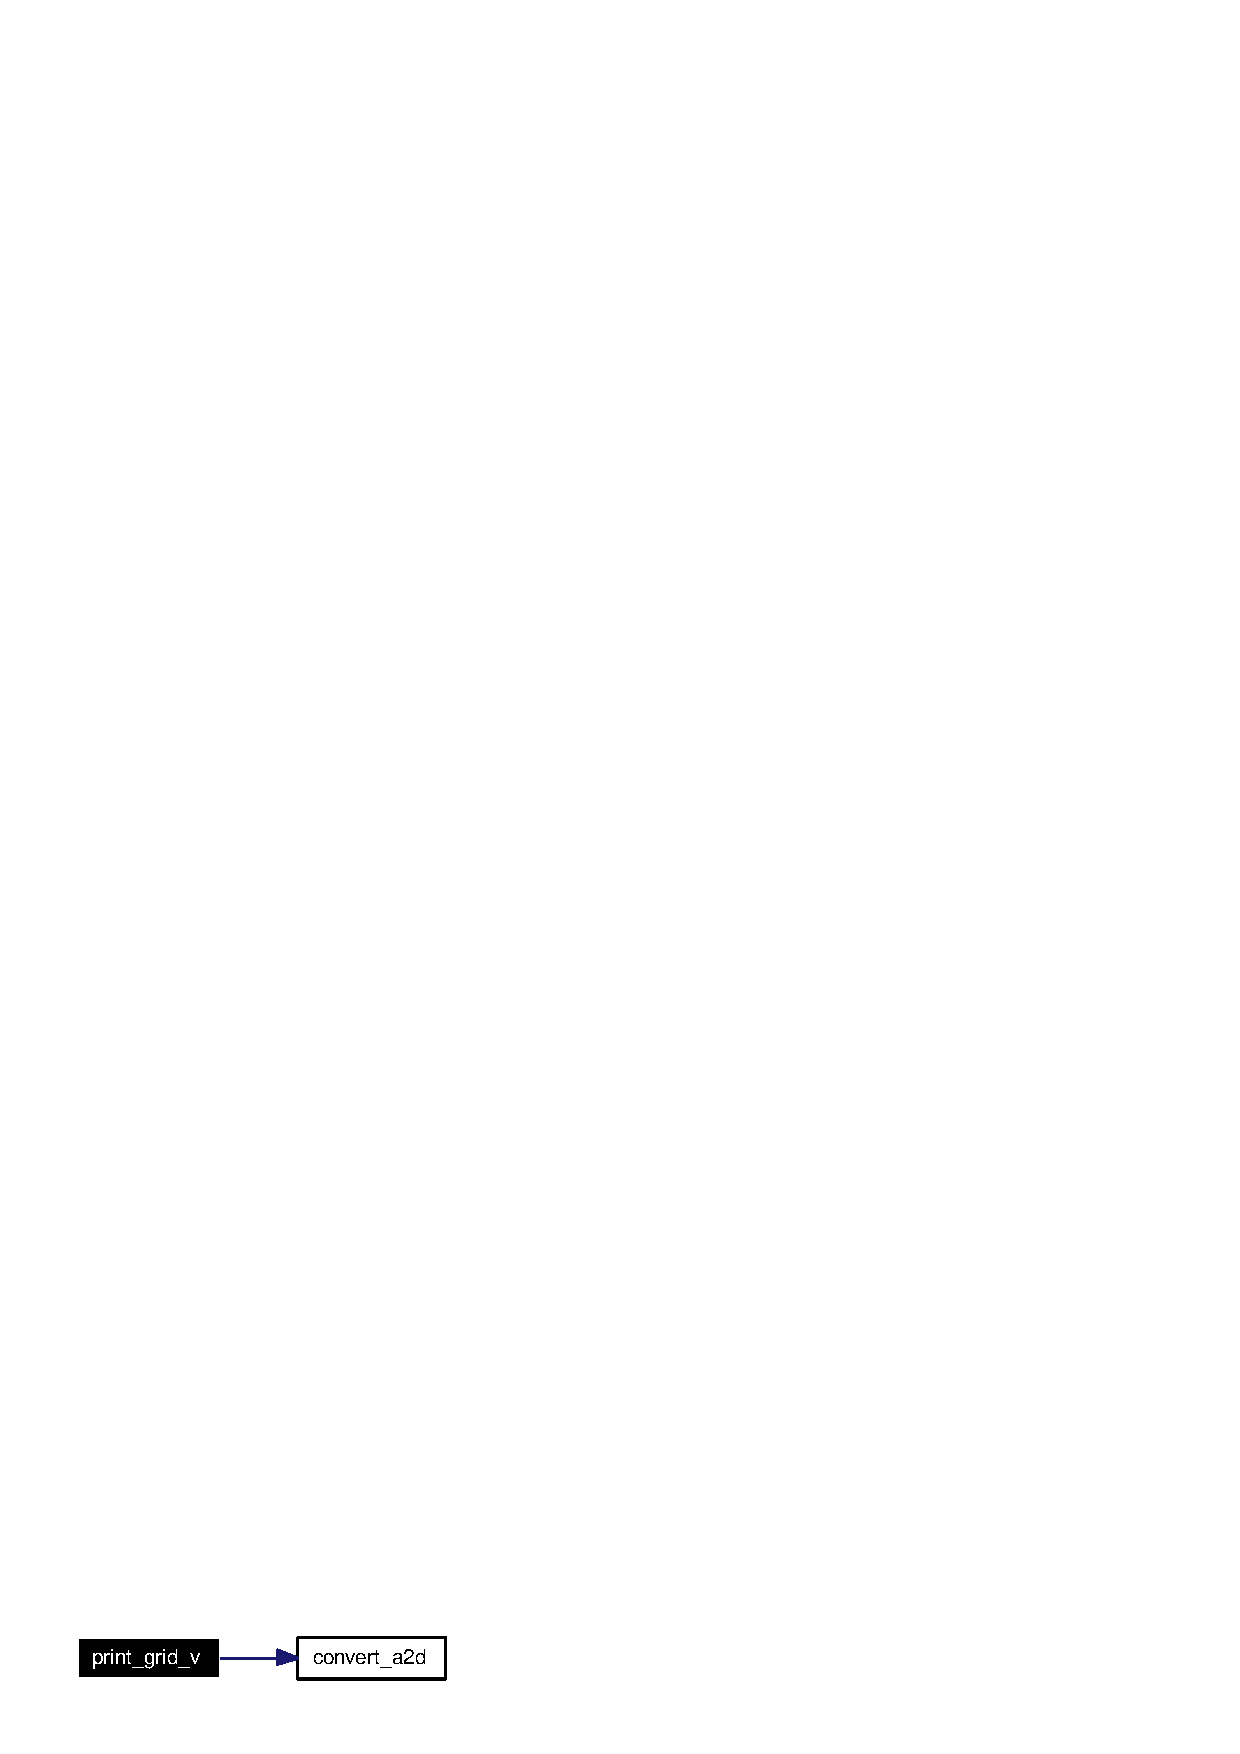
\includegraphics[width=107pt]{main_8c_a1_cgraph}
\end{center}
\end{figure}
\index{main.c@{main.c}!scan_probes@{scan\_\-probes}}
\index{scan_probes@{scan\_\-probes}!main.c@{main.c}}
\subsubsection{\setlength{\rightskip}{0pt plus 5cm}void scan\_\-probes ()}\label{main_8c_a5}




Definition at line 113 of file main.c.

References conversion\_\-result, convert\_\-a2d(), delay\_\-1\_\-25m\-S(), I\_\-CONVERSION, ueacval::integer, pin\_\-data, write\_\-current(), and write\_\-lla().

\footnotesize\begin{verbatim}113                    {
114   int i,j;
115   for (i=0;i<25;i++) {
116     write_lla(i,1);
117     printf("%d ",i);
118     for (j=200;j>=0;j-=50) {
119       write_current(i,j);
120       delay_1_25mS(400);     
121       convert_a2d(I_CONVERSION,pin_data[i].filtered_result,&conversion_result,i);
122       printf("%d ",conversion_result.integer);
123     }
124     printf("\n\r");
125     write_lla(i,0);
126   }
127 }
\end{verbatim}\normalsize 




Here is the call graph for this function:\begin{figure}[H]
\begin{center}
\leavevmode
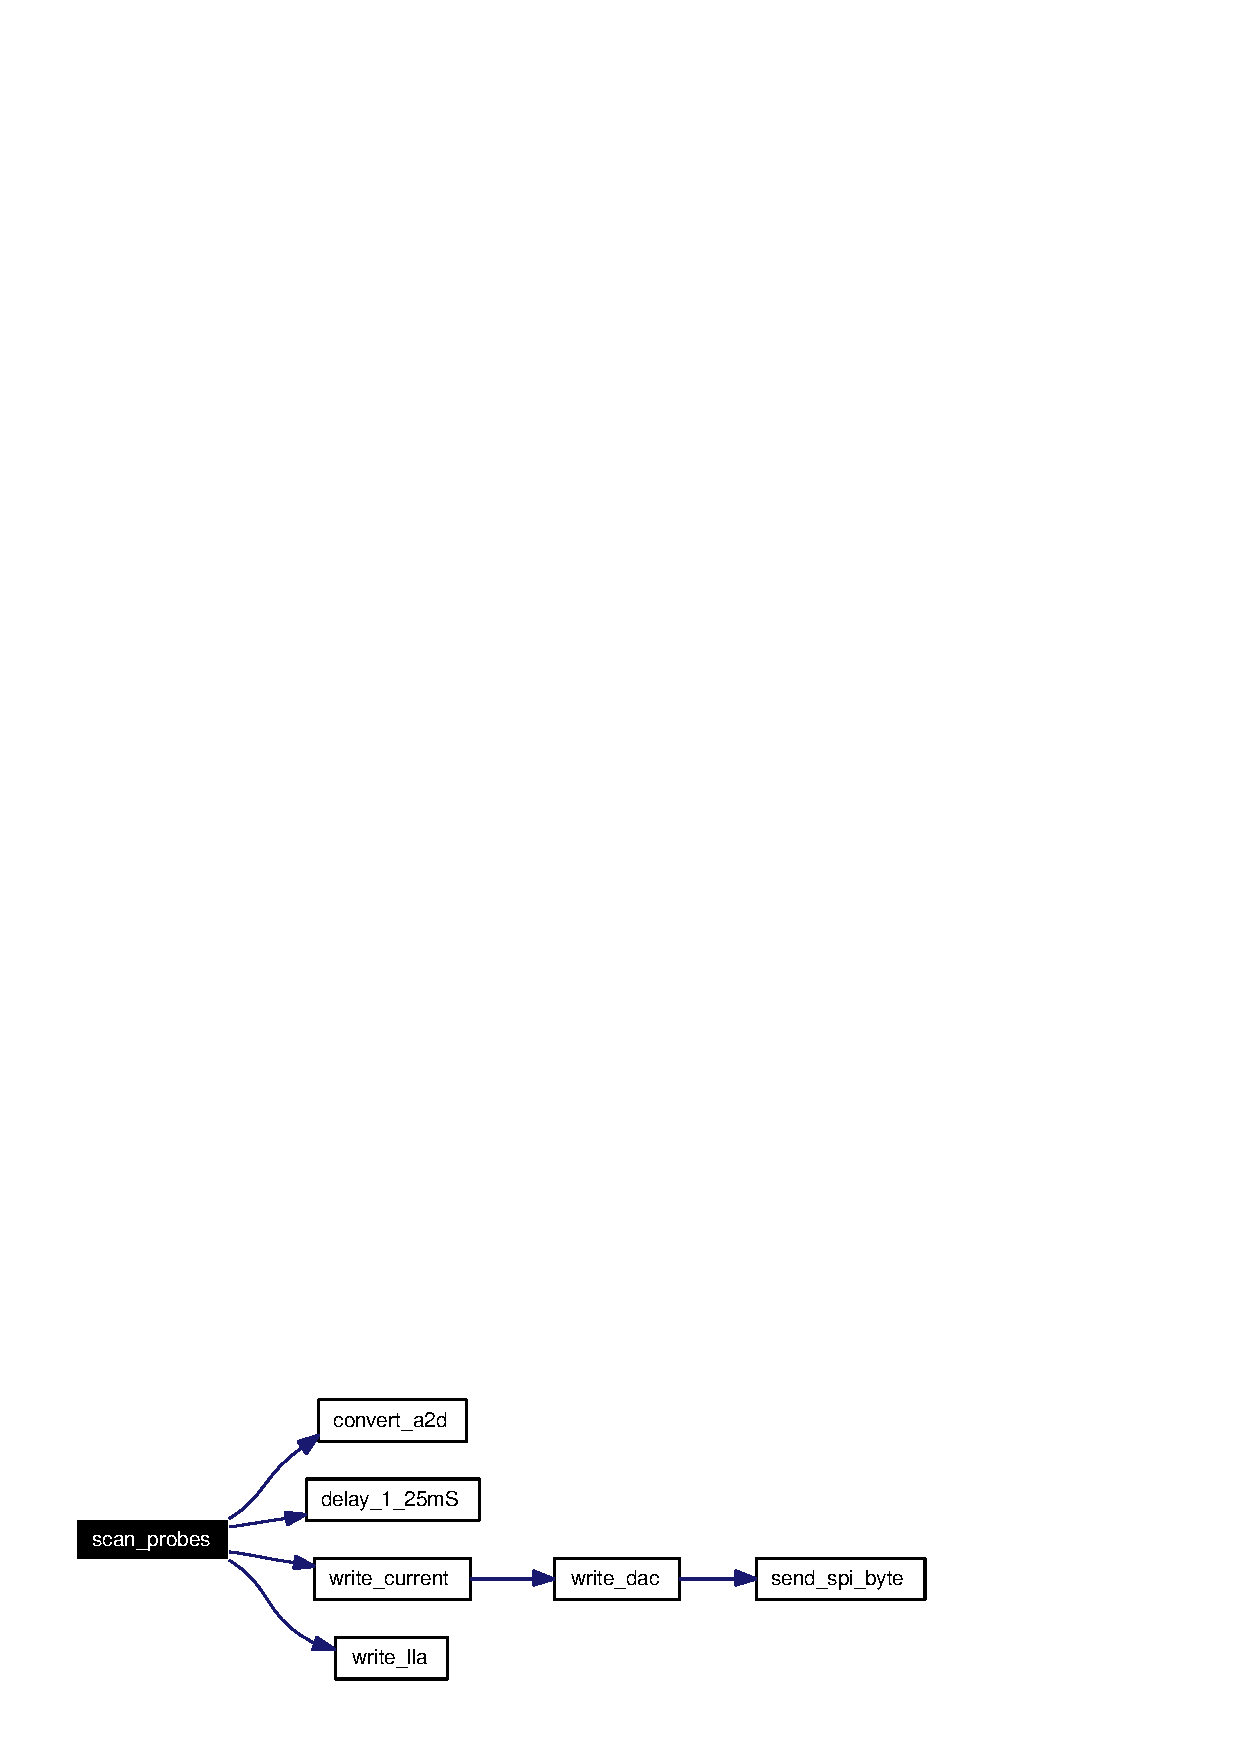
\includegraphics[width=222pt]{main_8c_a5_cgraph}
\end{center}
\end{figure}


\subsection{Variable Documentation}
\index{main.c@{main.c}!dac_translation@{dac\_\-translation}}
\index{dac_translation@{dac\_\-translation}!main.c@{main.c}}
\subsubsection{\setlength{\rightskip}{0pt plus 5cm}short {\bf dac\_\-translation}[$\,$]}\label{main_8c_a0}




Definition at line 45 of file cal\_\-table.h.